
% --------------------------------------------------------------
% This is all preamble stuff that you don't have to worry about.
% Head down to where it says "Start here"
% --------------------------------------------------------------

\documentclass[10pt]{article}

\usepackage[margin=.7in]{geometry}
\usepackage{amsmath,amsthm,amssymb}
\usepackage{enumitem}
\usepackage{tikz-cd}
\usepackage{mathtools}
\usepackage{amsfonts}
\usepackage{listings}
\usepackage{algorithm2e}
\usepackage{verse,stmaryrd}
\usepackage{fancyvrb}

% Number systems
\newcommand{\NN}{\mathbb{N}}
\newcommand{\ZZ}{\mathbb{Z}}
\newcommand{\QQ}{\mathbb{Q}}
\newcommand{\RR}{\mathbb{R}}
\newcommand{\CC}{\mathbb{C}}
\newcommand{\PP}{\mathbb P}
\newcommand{\FF}{\mathbb F}
\newcommand{\DD}{\mathbb D}
\renewcommand{\epsilon}{\varepsilon}

\newcommand{\Aut}{\operatorname{Aut}}
\newcommand{\coker}{\operatorname{coker}}
\newcommand{\CVect}{\CC\operatorname{-Vect}}
\newcommand{\Cantor}{\mathcal{C}}
\newcommand{\D}{\mathcal{D}}
\newcommand{\card}{\operatorname{card}}
\newcommand{\dbar}{\overline \partial}
\DeclareMathOperator*{\esssup}{ess\,sup}
\newcommand{\GL}{\operatorname{GL}}
\newcommand{\Hom}{\operatorname{Hom}}
\newcommand{\id}{\operatorname{id}}
\newcommand{\Ind}{\operatorname{Ind}}
\newcommand{\Inn}{\operatorname{Inn}}
\newcommand{\interior}{\operatorname{int}}
\newcommand{\lcm}{\operatorname{lcm}}
\newcommand{\mesh}{\operatorname{mesh}}
\newcommand{\LL}{\mathcal L_0}
\newcommand{\Leb}{\mathcal{L}_{\text{loc}}^2}
\newcommand{\Lip}{\operatorname{Lip}}
\newcommand{\ppGL}{\operatorname{PGL}}
\newcommand{\ppic}{\vspace{35mm}}
\newcommand{\ppset}{\mathcal{P}}
\DeclareMathOperator{\proj}{proj}
\DeclareMathOperator*{\Res}{Res}
\newcommand{\Riem}{\mathcal{R}}
\newcommand{\RVect}{\RR\operatorname{-Vect}}
\newcommand{\Sch}{\mathcal{S}}
\newcommand{\SL}{\operatorname{SL}}
\newcommand{\sgn}{\operatorname{sgn}}
\newcommand{\spn}{\operatorname{span}}
\newcommand{\Spec}{\operatorname{Spec}}
\newcommand{\supp}{\operatorname{supp}}
\newcommand{\TT}{\mathcal T}
\DeclareMathOperator{\tr}{tr}

\DeclareMathOperator{\adj}{adj}
\DeclareMathOperator{\curl}{curl}

% Calculus of variations
\DeclareMathOperator{\pp}{\mathbf p}
\DeclareMathOperator{\zz}{\mathbf z}
\DeclareMathOperator{\uu}{\mathbf u}
\DeclareMathOperator{\vv}{\mathbf v}
\DeclareMathOperator{\ww}{\mathbf w}

% Categories
\newcommand{\Ab}{\mathbf{Ab}}
\newcommand{\Cat}{\mathbf{Cat}}
\newcommand{\Group}{\mathbf{Group}}
\newcommand{\Module}{\mathbf{Module}}
\newcommand{\Set}{\mathbf{Set}}
\DeclareMathOperator{\Fun}{Fun}
\DeclareMathOperator{\Iso}{Iso}

% Complex analysis
\renewcommand{\Re}{\operatorname{Re}}
\renewcommand{\Im}{\operatorname{Im}}

% Logic
\renewcommand{\iff}{\leftrightarrow}
\newcommand{\Henkin}{\operatorname{Henk}}
\newcommand{\PA}{\mathbf{PA}}
\DeclareMathOperator{\proves}{\vdash}

% Group
\DeclareMathOperator{\Gal}{Gal}
\DeclareMathOperator{\Fix}{Fix}
\DeclareMathOperator{\Out}{Out}

% Other symbols
\newcommand{\heart}{\ensuremath\heartsuit}

\DeclareMathOperator{\atanh}{atanh}

% Theorems
\theoremstyle{definition}
\newtheorem*{corollary}{Corollary}
\newtheorem*{falselemma}{Grader's ``Lemma"}
\newtheorem{exer}{Exercise}
\newtheorem{lemma}{Lemma}[exer]
\newtheorem{theorem}[lemma]{Theorem}


\usepackage[backend=bibtex,style=alphabetic,maxcitenames=50,maxnames=50]{biblatex}
\renewbibmacro{in:}{}
\DeclareFieldFormat{pages}{#1}

\begin{document}
\noindent
\large\textbf{Fluid dynamics, HW 1} \hfill \textbf{Aidan Backus} \\
% --------------------------------------------------------------
%                         Start here
% --------------------------------------------------------------\

I talked about these problems with Tai Gobetti Borges.

\begin{exer}
Let $u$ be a velocity field, $X$ the flow map of $u$.
Show that the Jacobian $J(a, t) = \det \nabla X(a, t)$ satisfies
$$\frac{\partial J}{\partial t}(a, t) = J(a, t)(\nabla \cdot u)(X(a, t), t).$$
\end{exer}

Let us first recall
$$\frac{\partial \det}{\partial v^i}(v) = 1$$
whenever $v = (v^1, \dots, v^d)$ is a matrix; this holds because linearity of the determinant in each of the columns implies that $\partial_{v_i} \det$ is constant, and then we can take $v = 1$, for which the claim is clear.
Let us write $X = (X^1, \dots, X^d)$, and then
$$\frac{\partial J}{\partial t} = \sum_{i=1}^d \frac{\partial \det}{\partial X^i}(X) \det(\nabla \overline X_i) = \sum_{i=1}^d \det(\nabla \overline X_i)$$
where $\overline X_i^j = X^j$ if $i \neq j$ and $\overline X_i^i = \partial_t X^i = u^i(X)$, so
$$(\nabla \overline X_i)^{jk} = \begin{cases}
\partial_{a_k} u^j(X), &i = j\\
\partial_{a_k} X^j, &i \neq j.
\end{cases}$$
Thus
$$(\nabla \overline X_j)^{jk} = \frac{\partial}{\partial a_k}(u^j(X)) = \sum_{\ell=1}^d \frac{\partial u^j}{\partial x_\ell}(X) \frac{\partial X^\ell}{\partial a_k}.$$
So by multilinearity
$$\det(\nabla \overline X_i) = \frac{\partial u^i}{\partial x_i} \det(\nabla X)$$
which implies
$$J' = (\nabla \cdot u)(X) J$$
as desired.

\begin{exer}
Let $\Omega \subseteq \RR^3$ be open with $\partial \Omega$ smooth. Let $n$ be its outer unit normal field, and let $\omega$ be the vorticity of a velocity field.
Let $\psi$ be the stream function associated to $\omega$. Show that $\curl \psi \cdot n = 0$.
\end{exer}

Let $Z = \{x \in \RR^3: x_3 = 0\}$.
Since $\partial \Omega$ is smooth and $\RR^3$ is orientable, $\overline \Omega$ is an orientable smooth manifold with boundary.
So there is a smooth atlas $\mathcal W$ of $\overline \Omega$ such that:
\begin{enumerate}
\item For every $(W, \psi) \in \mathcal W$,
$$\psi(W \cap \partial \Omega) \subseteq Z.$$
\item For every $(W, \psi) \in \mathcal W$, $\psi$ is orientation-preserving.
\end{enumerate}
That is, $\mathcal W$ ``flattens out the boundary" of $\Omega$ while preserving parity.
Let us fix $(W, \psi) \in \mathcal W$ and prove that
$$\curl \psi\cdot n|W \cap \partial \Omega = 0.$$
Since $W$ was arbitrary, this implies $\curl \psi \cdot n = 0$.

Since $\psi$ is orientation-preserving and
\begin{equation}
\label{coordinate invariant curl}
(\curl F)^\flat = *(dF^\flat)
\end{equation}
for any vector field $F$ (where $\flat$ is induced by the trivial Riemannian metric and $*$ is the Hodge star), curl commutes with the pushforward map $\psi_*$; therefore it is no loss of generality to assume that $\psi$ is the identity, whence $W \cap \partial \Omega \subseteq Z$.
In that case, $n|W \cap \partial \Omega = \pm e_3$, where $e_3$ is the third unit vector; without loss of generality assume that $n|W \cap \partial \Omega = e_3$.

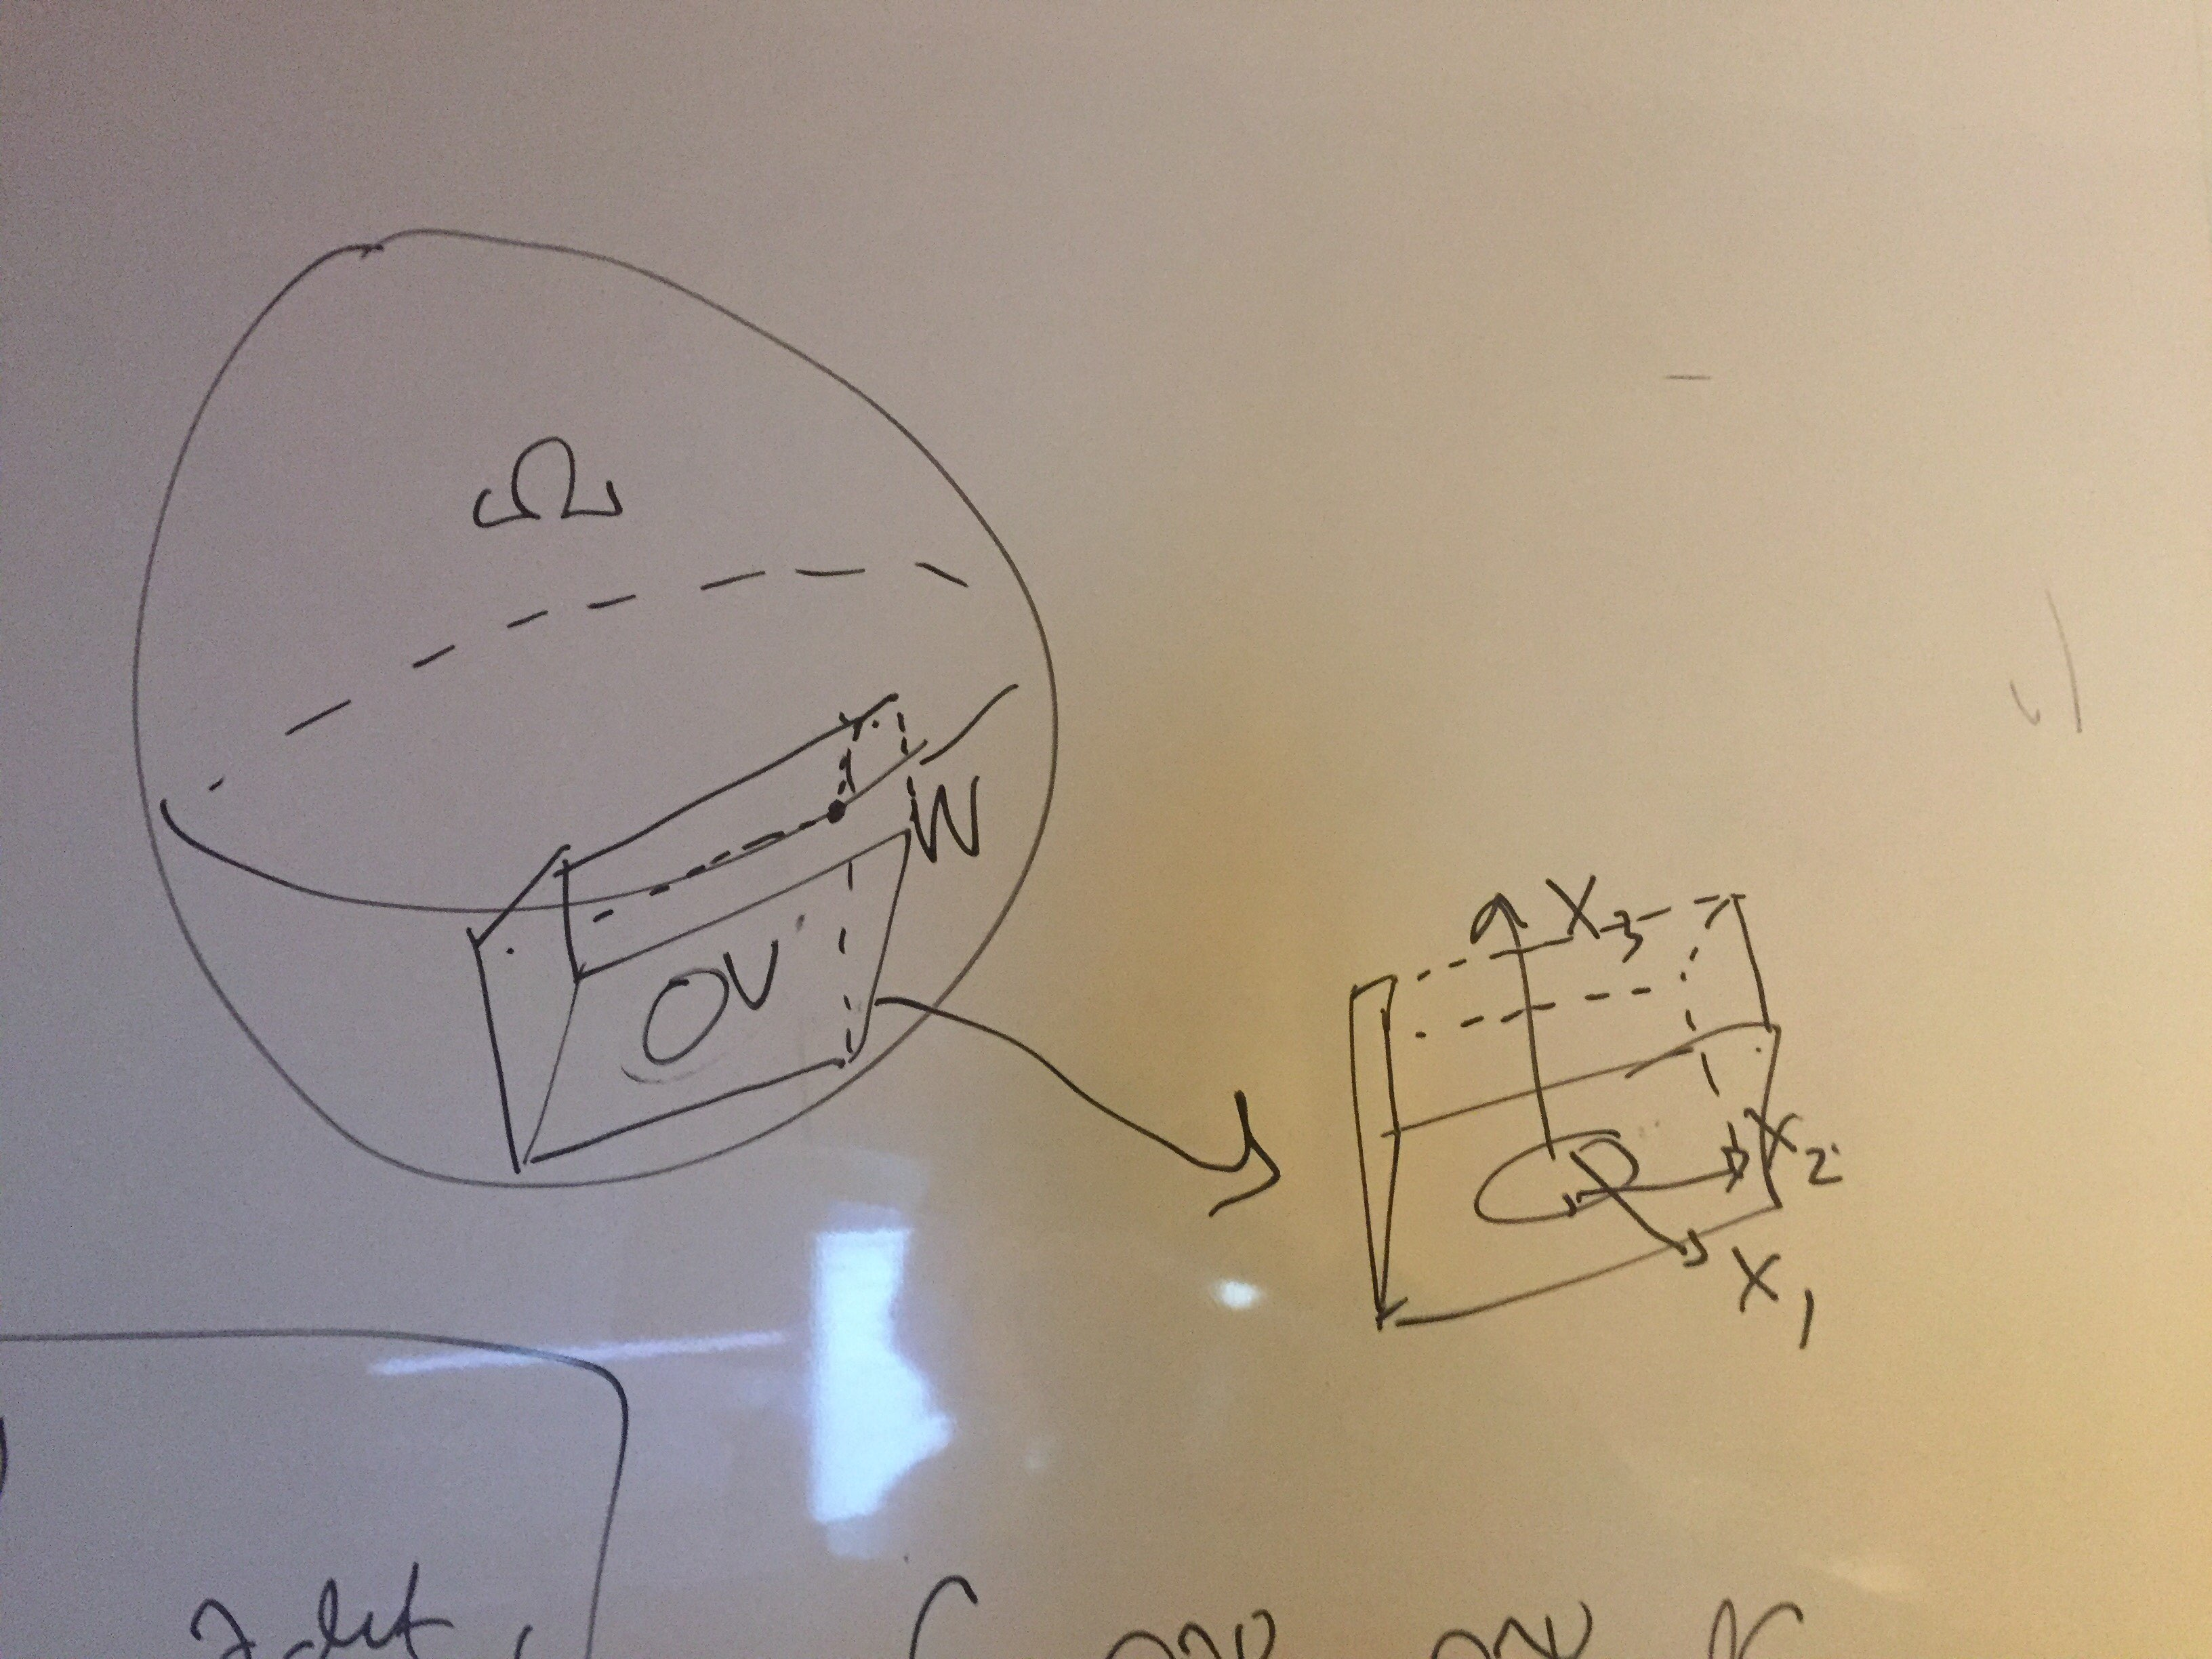
\includegraphics[scale=0.07]{fluids_1_coords.jpg}

Let $x \in W \cap Z$ and $\varepsilon > 0$. Let $V = \{y \in W \cap Z: |x - y| < \varepsilon\}$.
If $\varepsilon$ is small enough, then $V$ is a disk and $\partial V$ is a circle in $W \cap Z \subseteq \partial \Omega$.
Moreover,
$$\curl \psi \cdot e_3 = \frac{\partial \psi_2}{\partial x_1} - \frac{\partial \psi_1}{\partial x_2}$$
in $W$, so
$$\int_V \curl \psi \cdot e_3 ~dS = \int_V \frac{\partial \psi_2}{\partial x_1} - \frac{\partial \psi_1}{\partial x_2} ~dS = \int_{\partial V} \psi_1 ~dx_1 + \psi_2 ~dx_2 = 0,$$
by Green's theorem and the fact that $\psi = 0$ on $\partial \Omega$, which contains $\partial V$.
Since $\varepsilon$ is arbitrary and $\psi$ is smooth, this implies that $\curl \psi \cdot e_3(x) = 0$.
Since $x$ is arbitrary, $\curl \psi \cdot n|W \cap Z = 0$, as desired.

\begin{exer}
Let $\Omega$ be the upper-half plane. Derive the Biot-Savart law
$$u(x, t) = \frac{1}{2\pi} \int_\Omega \left(\frac{(x - y)^\perp}{|x - y|^2} - \frac{(x - \overline y)^\perp}{|x - \overline y|^2}\right) \omega(y, t) ~dy$$
where $u$ is the velocity field of an incompressible fluid of vorticity $\omega$.
\end{exer}

Extending $u, \omega$ to vector fields on $\Omega \times \RR$ in the usual way, we need to solve the Dirichlet div-curl system
$$\begin{cases}
\nabla \cdot u &= 0\\
\curl u &= \omega\\
u|\partial \Omega &= 0.
\end{cases}$$
Using the fact that on divergence-free vector fields, $\curl \curl = -\Delta$, and on scalar fields, $\curl = \nabla^\perp$, this system simplifies to the Laplace system
\begin{equation}
\label{Dirichlet Laplace}
-\Delta u = \nabla^\perp \omega
\end{equation}
with Dirichlet boundary condition.
Let $K_2$ be the Newtonian potential of $\RR^2$,
$$K_2(x) = -\frac{\log|x|}{2\pi}.$$
Solving the Laplace equation
$$
\begin{cases}-\Delta_y G(x, y) &= \delta(x - y)\\
G(x, y)|\RR^2 \times \partial \Omega &= 0
\end{cases}$$
we conclude that the integral kernel $G$ of $\Delta^{-1}$ with Dirichlet boundary condition is
$$G(x, y) = K_2(x - y) - K_2(x - \overline y).$$
The solution to the Dirichlet problem of the Laplace system (\ref{Dirichlet Laplace}) is
$$u(x, t) = \int_\Omega \nabla^\perp \omega(y, t) G(x, y) ~dy.$$
Integrating by parts and using the fact that $G|\partial \Omega = 0$ we conclude that
$$u(x, t) = -\int_\Omega \nabla^\perp_y G(x, y) \omega(y, t) ~dy.$$
It remains to compute $-\nabla^\perp G$. In fact,
\begin{align*}-\nabla^\perp_y G(x, y) &=
\frac{1}{2\pi} \left(\frac{\partial}{\partial y_2} \left(\frac{1}{\log|x - y|} - \frac{1}{\log|x - \overline y|}\right), \frac{\partial}{\partial y_1} \left(\frac{1}{\log|x - \overline y|} - \frac{1}{\log|x - y|}\right) \right)\\
&= \frac{1}{2\pi} \left(\frac{(y_2 - x_2, x_1 - y_1)}{|x - y|^2} - \frac{(x_2 + y_2, x_1 - y_1)}{|x - \overline y|^2}\right)
\end{align*}
while
$$\frac{(x - y)^\perp}{|x - y|^2} - \frac{(x - \overline y)^\perp}{|x - \overline y|^2} = \frac{(y_2 - x_2, x_1 - y_1)}{|x - y|^2} - \frac{(x_2 + y_2, x_1 - y_1)}{|x - \overline y|^2}$$
so this was as desired.

\begin{exer}
Prove that if $u = (f, 0)$ solves the Navier-Stokes equations with viscosity $\nu > 0$ in $\RR^2$ then the pressure is null and $f: \RR^{1 + 1} \to \RR$ solves the heat equation on $\RR$ with diffusivity $\nu$.
\end{exer}

Since $u$ is incompressible, we immediately have $\partial_y f = 0$. Therefore
$$(u \cdot \nabla)u = \left(f\frac{\partial f}{\partial y}, 0\right) = 0.$$
So the Navier-Stokes equations simplify to
\begin{equation}
\label{parabolic 1}
\frac{\partial f}{\partial t} + \frac{\partial p}{\partial y} = \nu \frac{\partial^2 f}{\partial y^2}.
\end{equation}
It remains to eliminate the pressure. In fact, if we take the gradient of the Navier-Stokes equations
$$\frac{\partial u}{\partial t} + (u \cdot \nabla)u + \nabla p = \nu \Delta u,$$
and write $U = (\partial_j u^i)_{ij}$, $P = (\partial_j \partial_i p)_{ij}$, we have
$$\frac{DU}{Dt} + U^2 + P = \nu \Delta U.$$
Taking traces and recalling $\nabla \cdot u = 0$ we get
$$\Delta p = \frac{\partial u^1}{\partial x_1} \frac{\partial u^2}{\partial x_2} + \frac{\partial u^2}{\partial x_1} \frac{\partial u^1}{\partial x_2} = 0.$$
On the other hand, since $p$ does not depend on its second coordinate (since $u = (f, 0)$), it must be the case that $\partial_{x_2}^2 p = 0$.
Therefore $p$ is a linear function of $x_1 = y$, so $\partial_y p$ is a constant, say $\kappa$, and the parabolic PDE (\ref{parabolic 1}) simplifies to
$$\frac{\partial f}{\partial t} + \kappa = \nu \frac{\partial^2 f}{\partial y^2}.$$
But since we assume that the pressure decays rapidly at infinity (say, $p$ is Schwartz), it must be the case that $\kappa = 0$, which gives the claim.

\begin{exer}
Let $u$ be a smooth, rapidly decaying solution of the Euler equations in $\RR^3$.
Show that the quantities $\int_{\RR^3} u(t)$, $\int_{\RR^3} \omega(t)$, and $\int_{\RR^3} u(t) \cdot \omega(t)$ are conserved in time.
\end{exer}

Let us first recall that if $f$ is a (say, Schwartz) scalar field
\begin{equation}
\label{integration by parts}
\int_{\RR^3} \nabla f = 0,
\end{equation}
an immediate consequence of the Stokes formula $\int_M df + \int_{\partial M} f = 0$ for Riemannian manifolds $M$.
Moreover,
$$\int_{\RR^3} (u \cdot \nabla)f = \int_{\RR^3} \sum_{i=1}^3 u^i \frac{\partial f}{\partial x_i} = - \int_{\RR^3} \sum_{i=1}^3 \frac{\partial u^i}{\partial x_i} f = -\int_{\RR^3} (\nabla \cdot u)f,$$
thus, since $u$ is incompressible,
\begin{equation}
\label{incompressible material}
\int_{\RR^3} (u \cdot \nabla)f = 0.
\end{equation}
Using (\ref{integration by parts}) on $f = p$ and (\ref{incompressible material}) on $f = u^j$, and the Euler equations, we get
$$\frac{\partial}{\partial t} \int_{\RR^3} u(t, x) ~dx = \int_{\RR^3} \frac{\partial u}{\partial t}(t, x) ~dx = -\int_{\RR^3} (u \cdot \nabla)u(t, x) - \nabla p(t, x) ~dx = 0.$$
Taking the curl of the resulting conservation of velocity flux
$$\frac{\partial}{\partial t} \int_{\RR^3} u(t, x)~dx = 0$$
we get the conservation of vorticity flux
$$\frac{\partial}{\partial t} \int_{\RR^3} \omega(t, x) ~dx = 0.$$

Now for conservation of helicity we recall the cyclicity formula
$$\alpha \cdot (\beta \times \gamma) = \beta \cdot (\gamma \times \alpha)$$
which combined with the fact that $\nabla \times F = \curl F$ we get the identity
\begin{equation}
\label{curl and divergence}
F \cdot \curl G + \nabla \cdot(F \times G) = 0.
\end{equation}
Multiplying the Euler equation
$$\frac{\partial u}{\partial t} + (u \cdot \nabla)u + \nabla p = 0$$
by the vorticity $\omega$ we get
$$\frac{\partial u}{\partial t} \cdot \omega + (u \cdot \nabla)u \cdot \omega + \nabla p \cdot \omega = 0.$$
Applying (\ref{curl and divergence}),
$$\nabla \cdot \left(\frac{\partial u}{\partial t} \times u\right) + \nabla \cdot ((u \cdot \nabla)u \times u) + \nabla \cdot (\nabla p \times u) = 0.$$
But
$$\nabla \cdot \left(\frac{\partial u}{\partial t} \times u\right) = \frac{1}{2} \frac{\partial}{\partial t} \nabla \cdot(u \times u) = 0$$
which implies that
$$\nabla \cdot ((u \cdot \nabla)u \times u) + \nabla \cdot (\nabla p \times u) = 0.$$
Applying (\ref{curl and divergence}) again we conclude that
$$((u \cdot \nabla)u + \nabla p) \cdot \omega = 0.$$
Thus, the product rule and the Euler equation implies
$$\frac{\partial}{\partial t} \int_{\RR^3} u \cdot \omega = \int_{\RR^3} u \cdot \frac{\partial \omega}{\partial t}.$$
Using the inviscid vorticity equation
$$\frac{\partial \omega}{\partial t} + (u \cdot \nabla)\omega = (\omega \cdot \nabla)u,$$
we deduce
$$\frac{\partial}{\partial t} \int_{\RR^3} u \cdot \omega = \int_{\RR^3} u \cdot \left((u \cdot \nabla)\omega - (\omega \cdot \nabla)u\right).$$
Since $u$ is incompressible,
\begin{align*}
\int_{\RR^3} u \cdot (u \cdot \nabla)\omega
&= \int_{\RR^3} \sum_{i,j=1}^3 u^ju^i\frac{\partial \omega_j}{\partial x_i}
= -\int_{\RR^3} \sum_{i,j=1}^3 \frac{\partial(u^ju^i)}{\partial x_i} \omega_j \\
&= -\int_{\RR^3} \sum_{i,j=1}^3 \frac{\partial u^j}{\partial x_i} u^i \omega_j - \int_{\RR^3} (\nabla \cdot u)\sum_{j=1}^3 u^j \omega_j\\
&= -\int_{\RR^3} \sum_{i,j=1}^3 \frac{\partial u^j}{\partial x_i} u^i \omega_j.
\end{align*}
Since $\omega$ is a curl, it is incompressible, so a similar argument shows
$$\int_{\RR^3} u \cdot (\omega \cdot \nabla)u = -\int_{\RR^3} \sum_{i,j=1}^3 \frac{\partial u^j}{\partial x_i} u^j \omega_i.$$
It follows that
$$\int_{\RR^3} u \cdot \left((u \cdot \nabla)\omega - (\omega \cdot \nabla)u\right) = 0$$
which completes the proof that helicity is conserved.

\begin{exer}
Let $u$ be a smooth, rapidly decaying solution of the Euler equations, $d = 2$, $p \in [1, \infty]$ and $\omega = \curl u$.
Show that the second moment $\int_{\RR^2} |x|^2 \omega(t, x) ~dx$ and the norm $||\omega(t)||_{L^p}$ of the vorticity are conserved, using the conservation of vorticity along streamlines.
\end{exer}

Since $d = 2$, $\omega$ is a scalar field which is constant along streamlines, thus
\begin{equation}
\label{streamline invariance}
\frac{\partial \omega}{\partial t} + (u \cdot \nabla)\omega = 0.
\end{equation}
To bound the time derivative of the second moment, we will let $(t, x, y)$ be the usual spacetime coordinates on $\RR^{1+2}$, $dA = dx \wedge dy$, $u = (u_x, u_y)$.
Let $\varepsilon > 0$.
We claim that
\begin{equation}
\label{second moment changes slowly}
\left|\frac{\partial}{\partial t} \iint_{\RR^2} (x^2 + y^2) \omega ~dx \wedge dy\right| \lesssim \varepsilon
\end{equation}
which implies the claim as $\varepsilon \to 0$.
(Let us assume that ``rapidly decaying" means Schwartz, though this argument can be adapted to similar decay conditions.)
By (\ref{streamline invariance}) and an integration by parts, we have
\begin{align*}
\frac{\partial}{\partial t} \iint_{\RR^2} (x^2 + y^2) \omega ~dA &=
-\iint_{\RR^2} (x^2 + y^2)\left(u_x \frac{\partial \omega_x}{\partial x} + u_y \frac{\partial \omega_y}{\partial y}\right) ~dA\\
&= \iint_{\RR^2} \left[\left(\frac{\partial}{\partial x} u_x + \frac{\partial}{\partial y} u_y\right)(x^2 + y^2)\right] \omega~dA.
\end{align*}
(Here the differential operator $\partial_x u_x + \partial_y u_y$ is just acting on $x^2 + y^2$.)

Now introduce the differential $1$-form $\alpha = u^\flat$. Explicitly, $\alpha = u_x ~dx + u_y ~dy$.
By the coordinate-free definition of the curl (\ref{coordinate invariant curl}), $d\alpha = \omega ~dA$.
So
\begin{align*}
\frac{\partial}{\partial t} \iint_{\RR^2} (x^2 + y^2) \omega ~dA &= \iint_{\RR^2} \left(\frac{\partial}{\partial x} u_x + \frac{\partial}{\partial y} u_y\right)(x^2 + y^2) ~d\alpha\\
&= \iint_{\RR^2} \left((\nabla \cdot u)\cdot(x^2 + y^2) + 2(xu_x + yu_y)\right) ~d\alpha\\
&= 2\iint_{\RR^2} (xu_x + yu_y) ~d\alpha
\end{align*}
owing to the incompressibility $\nabla \cdot u = 0$.
Then we can let $\beta = (xu_x + yu_y) ~d\alpha$.
Since $\beta$ is a $2$-form on the contractible surface $\RR^2$, there is a $1$-form $\gamma$ such that $d\gamma = \beta$.

Since $u$ is Schwartz, so are the components of $\beta$, so there is a compact set $K$ such that $\iint_{K^c} |\beta| < \varepsilon$.
Let $U$ be an open set that contains $K$ such that $\partial U$ is smooth and let $\chi$ be a smooth cutoff such that $\chi|K = 1$ and $\chi|U^c = 0$.
Then, in particular,
$$\left|\iint_{K^c} \chi\beta\right| < \varepsilon$$
so it is no loss of generality towards the bound (\ref{second moment changes slowly}) to assume that $\beta = \chi\beta$ and thus $\beta$ is supported in $K$. But then $\gamma|\partial U = 0$, so
$$\iint_U \beta = \int_{\partial U} \gamma = 0.$$
This completes the proof of (\ref{second moment changes slowly}).

Now for the norm, which is much easier.
First assume that $p < \infty$.
Since $u$ is incompressible, Exercise 1 shows that the Jacobian $J(t, x)$ of the action of the one-parameter group $X$ is constant in $t$.
But for any $x$, $J(0, x) = 1$, since $0$ is the identity; therefore $J = 1$ identically.
So for any $s \in \RR$,
$$\int_{\RR^2} |\omega(t, x)|^p ~dx = \int_{\RR^2} |\omega(t, X(s, x))|^p ~dx.$$
In particular this holds when $s = t$. But since $u$ is $X$-invariant by (\ref{streamline invariance}),
$$\omega(t, X(t, x)) = \omega(0, x).$$
That implies
$$\int_{\RR^2} |\omega(t, x)|^p ~dx = \int_{\RR^2} |\omega(0, x)|^p ~dx$$
which does not depend on $t$.
By continuity, then, this argument extends to $p = \infty$.

\end{document}
